%Autor: Simon Walker
%Version: 1.0
%Datum: 16.12.2019

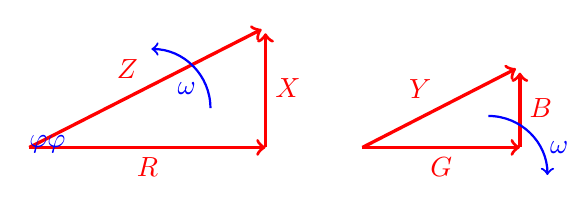
\begin{tikzpicture}


	\coordinate (A1) at (0,0);
	\coordinate (R1) at (3,0);
	\coordinate (X1) at (3, 1.5);
	
	\draw[red, ->, very thick] (0, 0) -- (3, 0);
	\node[red, below] at (1.5, 0) {$R$};
	
	\draw[red, ->, very thick] (3, 0) -- (3, 1.45);
	\node[red, right] at (3, 0.75) {$X$};
	
	\draw[red, ->, very thick] (0, 0) -- (2.95, 1.5);
	\node[red, above left] at (1.5, 0.75) {$Z$};
	
	\draw[blue, ->, thick] (2.3, 0.5) arc (0:90:0.75);
	\node[blue] at (2, 0.75){$\omega$};
	
	\markangle[blue]{X1}{A1}{R1}{$\textcolor{blue}{\varphi}$}{12};
	
	\coordinate (A2) at (4,0);
	\coordinate (R2) at (6,0);
	\coordinate (X2) at (6, 1);
	
	\draw[red, ->, very thick] (4, 0) -- (6, 0);
	\node[red, below] at (5, 0) {$G$};
	
	\draw[red, ->, very thick] (6, 0) -- (6, 0.95);
	\node[red, right] at (6, 0.5) {$B$};
	
	\draw[red, ->, very thick] (4, 0) -- (5.95, 1);
	\node[red, above left] at (5, 0.5) {$Y$};
	
	\draw[blue, ->, thick] (5.6, 0.4) arc (90:0:0.75);
	\node[blue] at (6.5, 0){$\omega$};
	
	\markangle[blue]{X2}{A2}{R2}{$\textcolor{blue}{\varphi}$}{12};
	
	%\HelpCords{0}{0}{8}{3}
\end{tikzpicture}
